\chapter{人口学特征}

\section{年龄}

《尚未实现》

\section{文化程度}

育龄夫妇的教育水平关系到孕前优生宣传教育开展的效果,教育水平的高低不仅与危险因素的暴露比例密切相关,而且对于成功开展孕前优生健康检查及出生缺陷一级预防至关重要。

统计结果显示,2015年广东省深圳市参加检查的服务对象受教育水平普遍较高。男性参检服务对象中,《尚未支持排序,3个》大专/大本人群占None/{{sql=select count(*) from exam where service\_code like '4403\%' and complete=1 and medu\_level is not null and service\_time between '2015-01-01' and '2015-12-31'}}*100}}\%,其次为高中/中专/中技(16.30\%),初中(7.82\%),研究生及以上教育水平者也占到6.47\%。全市及不同地区男性参检人群的受教育水平比例如下图所示。
\begin{figure}[htbp]
	\centering
	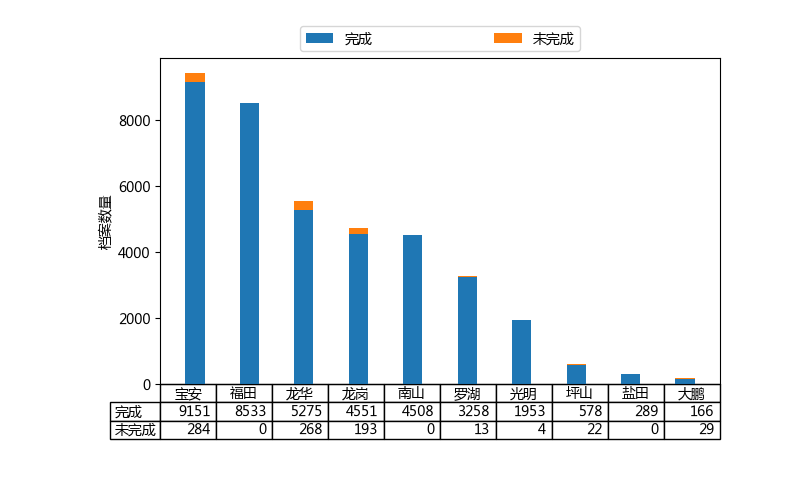
\includegraphics[width=1\textwidth]{1.png}
	\caption{测试图片}
	\label{图2}
\end{figure}




女性参检服务对象中,《尚未支持排序,3个》大专/大本的人群比例为None/{{sql=select count(*) from exam where service\_code like '4403\%' and complete=1 and fedu\_level is not null and service\_time between '2015-01-01' and '2015-12-31'}}*100}}\%,其次是高中/中专/中技所占比例17.21\%,初中比例为9.18\%,研究生及以上所占比例为5.05\%。全市及不同地区女性参检人群的受教育水平的构成如下图所示。
\begin{figure}[htbp]
	\centering
	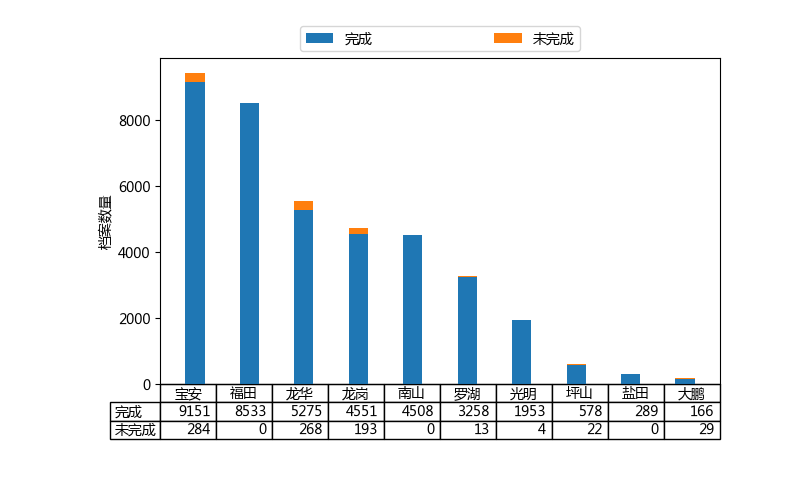
\includegraphics[width=1\textwidth]{1.png}
	\caption{测试图片}
	\label{图2}
\end{figure}




\section{职业构成}

2015年度广东省深圳市的参检人群中,参检男性服务对象的职业《尚未支持排序,3个》以教师/公务员/职员等为主,占参检对象(男性)总数的None/{{sql=select count(*) from exam where service\_code like '4403\%' and complete=1 and mjob is not null and service\_time between '2015-01-01' and '2015-12-31'}}*100}}\%,其次为工人,服务业,分别占22.77\%和9.56\%。全市和不同地区男性参检服务对象的职业构成情况如下图所示。



女性参检服务对象《尚未支持排序,3个》None/{{sql=select count(*) from exam where service\_code like '4403\%' and complete=1 and fjob is not null and service\_time between '2015-01-01' and '2015-12-31'}}*100}}\%中,54.04\%的参检对象职业为教师/公务员/职员等,其次是工人占女性参检人群的比例为21.47\%,服务业、家务和经商分别占10.05\%、5.30\%和4.37\%。各类型女性参检人群的比例构成如下图所示。





\section{民族构成}

2015年度广东省深圳市参加孕前优生健康检查的男性参检《尚未支持排序,5个》人群的民族以汉族为主,占总数的None/{{sql=select count(*) from exam where service\_code like '4403\%' and complete=1 and mnationality is not null and service\_time between '2015-01-01' and '2015-12-31'}}*100}}\%,其次壮族、土家族、苗族和满族,分别占0.61\%,0.32\%,0.26\%和0.21\%。各地区少数民族参检男性的参检比例如下图所示。



女性《尚未支持排序,5个》参检人群的民族也以汉族为主,占总数的None/{{sql=select count(*) from exam where service\_code like '4403\%' and complete=1 and fnationality is not null and service\_time between '2015-01-01' and '2015-12-31'}}*100}}\%,其次壮族、土家族、苗族和瑶族,分别占0.65\%、0.38\%、0.26\%和0.18\%。各地区少数民族参检女性的参检比例分布情况如下图所示。



\section{参检人群户籍情况}

2015年度,广东省深圳市全市参加孕前检查的人群中,男性参检人群(除去男方未签署知情同意书的)中非本地户籍的人群占None/{{sql=select count(*) from exam where service\_code like '4403\%' and complete=1 and has\_content between 3 and 4 and maccount\_location\_city is not null and address\_city is not null and service\_time between '2015-01-01' and '2015-12-31'}}*100}}\%。



女方参检人群(除去女方未签署知情同意书的)中非本地户籍人数占None/{{sql=select count(*) from exam where service\_code like '4403\%' and complete=1 and (has\_content=2 or has\_content=4) and faccount\_location\_city is not null and address\_city is not null and service\_time between '2015-01-01' and '2015-12-31'}}*100}}\%。全市及不同地区的参检人群中,不同户籍人口的参检比例如下图所示。

在夫妻双方共同参加(知情同意书为双方签署)检查的人群中,双方均为本地户籍的人群占None/{{sql=select count(*) from exam where service\_code like '4403\%' and complete=1 and has\_content between 3 and 4 and maccount\_location\_city is not null and faccount\_location\_city is not null and address\_city is not null and service\_time between '2015-01-01' and '2015-12-31'}}*100}}\%;双方均为外地户籍的人群占None/{{sql=select count(*) from exam where service\_code like '4403\%' and complete=1 and has\_content between 3 and 4 and maccount\_location\_city is not null and faccount\_location\_city is not null and address\_city is not null and service\_time between '2015-01-01' and '2015-12-31'}}*100}}\%;男方为本地户籍,女方为外地户籍的占None/{{sql=select count(*) from exam where service\_code like '4403\%' and complete=1 and has\_content between 3 and 4 and maccount\_location\_city is not null and faccount\_location\_city is not null and address\_city is not null and service\_time between '2015-01-01' and '2015-12-31'}}*100}}\%;男方为外地户籍,女方为本地户籍None/{{sql=select count(*) from exam where service\_code like '4403\%' and complete=1 and has\_content between 3 and 4 and maccount\_location\_city is not null and faccount\_location\_city is not null and address\_city is not null and service\_time between '2015-01-01' and '2015-12-31'}}*100}}\%。
